% Μεμονωμένο Παράρτημα 
% ορίζεται ο τίτλος του παραρτήματος
\edef\chaptertitle{Τίτλος Παραρτήματος}
\label{appendix}

% Μην τροποποιήσετε τις ακόλουθες εντολές
\chapter*{\chaptername\\\vspace{1cm} \chaptertitle} 
\addcontentsline{toc}{chapter}{\chaptername\texorpdfstring{\\}~\chaptertitle}
\setcounter{section}{0}
\renewcommand{\chaptermark}[1]{\markboth{\textit{\chaptername. \chaptertitle}}{}}
\chaptermark{}


Τα παραρτήματα περιλαμβάνουν συνοδευτικό, υποστηρικτικό υλικό (πίνακες, φωτογραφίες, ερωτηματολόγια, στατιστικά στοιχεία, αποδείξεις, περιγραφές  λογισμικών  προγραμμάτων,  παραδείγματα,  περιγραφές 
πολύπλοκων διαδικασιών, λίστα με πρωτογενή στοιχεία, λεπτομερής περιγραφή και προδιαγραφές εξοπλισμού, οδηγίες εγκατάστασης λογισμικού, κ.λπ.), ή αλλιώς ό,τι θεωρείται χρήσιμο να περιγραφεί, αλλά δεν συνηθίζεται να 
εντάσσεται μέσα στο κυρίως κείμενο της Εργασίας.  Στο κυρίως κείμενο της Εργασίας πρέπει να γίνονται οι κατάλληλες παραπομπές προς τα παραρτήματα, όπου το κείμενο σχετίζεται με υλικό που περιλαμβάνεται σε αυτά. Ένα παράρτημα, αναλόγως με το περιεχόμενό του, μπορεί να είναι ενιαίο, ή να χωρίζεται σε ενότητες.


\section{Δυνατότητες του \LaTeX}

Kαθώς το παρόν αποτελεί ένα πρότυπο συγγραφής διπλωματικών εργασιών, στην ενότητα αυτή επιδεικνύονται ορισμένες από τις δυνατότητες το \LaTeX οι οποίες μπορούν να αξιοποιηθούν στο κείμενο μιας διπλωματικής εργασίας (μια καλή πηγή για τη διερεύνηση των δυνατοτήτων του \LaTeX είναι η ιστοσελίδα {\small\url{https://www.overleaf.com/learn/latex/Main_Page}}).

\subsection{Πίνακες}
Ο Πίνακας~\ref{tab1} είναι ένα παράδειγμα πίνακα σχεδιασμένου με εντολές του περιβάλλοντος \texttt{tabular}.
\begin{table}[htb]
\centering
\caption{Παράμετροι πειραμάτων}
\label{tab1}
\begin{tabular}{|c|>{\centering\arraybackslash}m{8cm}|}
\hline Πλήθος κελιών καννάβου \textit{{c}} $\times$ \textit{{c}} & 50 $\times$ 50, 100 $\times$ 100, 200 $\times$ 200, \textbf{250} $\times$ \textbf{250}, 500 $\times$ 500, 1000 $\times$ 1000  \\
\hline Τυπική απόκλιση $\sigma$ & 25{m}, 50{m}, 75{m}, \textbf{100{m}}, 150{m}, 200{m} \\
\hline Αριθμός εγγύτερων γειτόνων \textit{{k}} & 1, 2, \textbf{3}, 4, 5, 10, 20 \\
\hline Πιθανοτικό κατώφλι $\theta$ & 50$\%$, 60$\%$, 70$\%$, \textbf{75$\%$}, 80$\%$, 90$\%$, 99$\%$ \\
\hline  
\end{tabular}

\end{table}

\subsection{Διαγράμματα - Γραφικές παραστάσεις}
Στο Σχήμα~\ref{fig1}, παρουσιάζεται ένα παράδειγμα γραφικής παράστασης σχεδιασμένης με το Gnuplot.
\begin{figure}[htb]
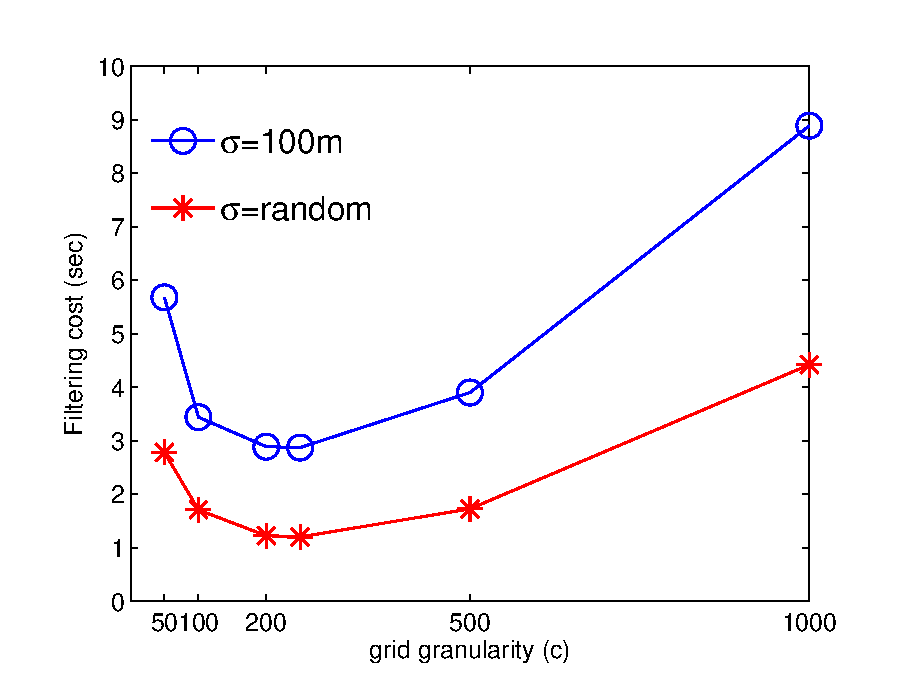
\includegraphics[scale=0.7]{figures/grid_granularity.eps}
\centering
\caption{Κλιμάκωση χρόνου εκτέλεσης για διάφορες υποδιαιρέσεις του καννάβου}	
\label{fig1}
\end{figure} 

\subsection{Σχήματα}
Ακολουθεί στο Σχήμα~\ref{fig2} ένα παράδειγμα σχήματος φτιαγμένου με εντολές του πακέτου Ti\textit{k}Z.
\begin{figure}[htb]
\begin{center}
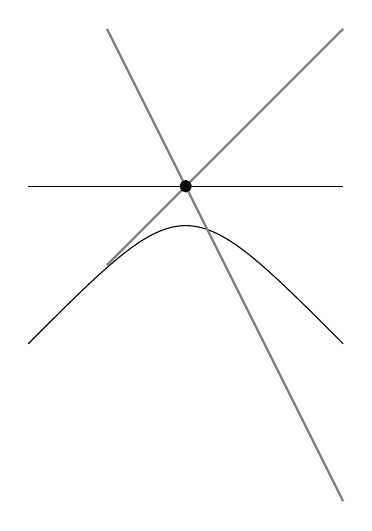
\begin{tikzpicture}
\draw (-2,0) -- (2,0);
\filldraw [gray] (0,0) circle (2pt);
\draw (-2,-2) .. controls (0,0) .. (2,-2);
%\draw (-2,2) .. controls (-1,0) and (1,0) .. (2,2);
 \draw[gray, thick] (-1,2) -- (2,-4);
\draw[gray, thick] (-1,-1) -- (2,2);
\filldraw[black] (0,0) circle (2pt)  ;
\end{tikzpicture}
\end{center}
\caption{Παράδειγμα σχήματος με εντολές του πακέτου Ti\textit{k}Z}	
\label{fig2}
\end{figure}

\subsection{Αλγόριθμοι}
Ακολουθεί ο Αλγόριθμος~\ref{alg1}, ο οποίος είναι μορφοποιημένος με τα πακέτα algorithm και algorithmic.

\begin{algorithm}[htb]
\caption{\ \ \ Probabilistic $k\theta NN$ Monitoring}
\begin{algorithmic}[1]
\begin{small}

\STATE{\bf Procedure} {\em VerifyCandidate} (focal query point $q$, threshold $\theta$, object $o$, list of auxiliary objects $P$, distance $kMAXDIST$) 

\IF { $\Phi(o, kMAXDIST) \geq \theta$ {\bf and} $L_2(q, o) \leq L_2(q, P.$top()) }

\STATE {$P$.pop()};   \ \ \ \ \ \ \ \ {\em //Replace the most extreme element in $P$, since candidate $o$ ... }

\STATE {$P$.push($o$)};  \ \ \ \ \ {\em //... has enough probability and has its mean closer to focal $q$ }

\ENDIF

\STATE {\bf End Procedure}


\end{small}
\end{algorithmic}
\label{alg1}
\end{algorithm}

\subsection{Μαθηματικές εκφράσεις}
Ακολουθούν παραδείγματα μαθηματικών εκφράσεων.
\begin{eqnarray}
\hat{I}(x,u,t)     &=& dist(y(t_f),\Gamma)
+  \int_t^{t_f} \: {\cal L}( y(s),u(s),s) \: ds
\label{con11b}
\end{eqnarray}

     \[
        \frac{d}{dx}\left( \int_{0}^{z} f(u)\,du\right)=f(x).
     \]

\subsection{Θεωρήματα, Πορίσματα, Ορισμοί, κλπ.}

Ακολουθεί παράδειγμα θεωρήματος από την ιστοσελίδα  {\small\url{https://www.overleaf.com/learn/latex/Theorems_and_proofs}}

\begin{theorem}
Let $f$ be a function whose derivative exists in every point, then $f$ 
is a continuous function.
\end{theorem}

\subsection{Απαριθμήσεις}

Μια απαρίθμηση (itemized list) βοηθά στην παρουσίαση μιας σειράς περιπτώσεων με σαφήνεια.
Ακολουθεί παράδειγμα.

H εκπαίδευση στην Ελλάδα διακρίνεται σε:
\begin{itemize}
\item Πρωτοβάθμια 
\item Δευτεροβάθμια 
\item Τριτοβάθμια 
\end{itemize}

\subsection{Είδη πηγών στις αναφορές}

Στο references.bib μπορεί να δει κανείς πώς γράφονται διάφορα είδη πηγών 
(Βιβλία Ξενόγλωσσα \cite{goossens93},
Βιβλία Ελληνικά \cite{greekbook},
Άρθρα σε επιστημονικά περιοδικά \cite{LiArTs13},
Άρθρα σε επιστημονικά συνέδρια \cite{dcis2011},
Ιστοσελίδες \cite{LaTeXProject},
Πτυχιακές Εργασίες \cite{elli05},
Διπλωματικές Εργασίες \cite{zoi04},
Μεταπτυχιακές Διπλωματικές Εργασίες \cite{master04},
Διδακτορικές Διατριβές \cite{phd045},
Τεχνικές Αναφορές \cite{MSU-CSE-05-29},
Διπλώματα Ευρεσιτεχνίας \cite{viswanathan2014convenient}),
Κεφάλαια σε συλλογικούς τόμους
\cite{[PS11]}.

